%% LyX 1.6.10 created this file.  For more info, see http://www.lyx.org/.
%% Do not edit unless you really know what you are doing.
\documentclass[english]{article}
\usepackage{babel}
\usepackage{amsmath}% mathtools includes this so this is optional
\usepackage{mathtools}
\usepackage{graphicx}
\usepackage{hyperref}

\begin{document}

\subsection*{Notes}

- References are still in pseudo format and need to be added
\newline \noindent
- It would be good to add a pseudo-code
\newline \noindent
- Note that our method only does identification of cloud cores, not tracking.
\newline \noindent
- The algorithm development profited from discussions with Mike Whitall (UK Met Office).
\newline \noindent
- The value of $f$ may need updating.
\newline \noindent
- I am still working on the literature section.
\newline \noindent
- Michael Whitall and I have some ideas on how to deal with tracking, splitting and merging as well, but this will need significant amounts of work.

\subsection*{Literature on cloud identification and tracking}

For studies of cloud processes, it is informative to regard processes in relation to the properties of the clouds, such as the cloud size distribution and the cloud lifecycle. Previous studies have developed methods for identifying and tracking clouds in both observations and simulations. The algorithm described below is concerned with the first of these issues, i.e. cloud identification, only. Though the design of tracking algorithms is not fully independent of the cloud identification algorithm, the current method could be combined with an existing tracking algorithm. 

Tracking in numerical data has been done by e.g. Zhao2005, Heus2009, Dawe2012 and Yu2016. For radar data, early tracking studies include the work of Austin1982 and Rosenfeld1985. Widely used methods for tracking in radar data include TITAN (e.g Dixon1993, Han2009), SCIT (Johnson1998) and TRACE3D (Handwerker2002). A particular problem in tracking are so-called false mergers (adjacent storms with weak connections). 

When identifying cloud regions, a simplification that significantly decreases the cost of the computation is to use two-dimensional fields (e.g. Heus2013). Two-dimensional techniques are somewhat limited in certain situations, e.g. when there is overlap between different cloud layers or shear. Clouds that consist of multiple transient updraughts (e.g. Heus2009) also present a challenge for cloud identification. One approach that is often taken is to further distinguish core regions (for example strong updraughts) and associate these with the clouds. One approach that can be used here is to introduce an additional criterion for cores (e.g. Dawe2012 and Heus2013), and associate the non-core regions with the cores. An alternative approach (Johnson1998, Yu2016) uses multiple thresholds. A key issue here is to identify which parts of the cloud belong to which core. Often, this is done by an iteratively growing the region around a core, but more sophisticated techniques exit (e.g. Yu2016).

The current algorithm is based on a three-dimensional topological analysis of the field. Similar, but more generic techniques exist in the literature on computational geometry (e.g. Carr2003). Techniques based on computational geometry have been used analyse volcanic plumes (e.g. Kuhn2015). 

The algorithm has been written in C++, and aims to minimise memory footprint. Part of this is to represent the data as 16-bit integers. In order to do this, the data is internally represented using a non-linear transform. Given e.g. the vertical velocity field $w$, its internal representation $\tilde{w}$ is given by:

\begin{equation}
\tilde{w}=\text{int} \left( 3200 \sqrt{\lvert w \rvert} {\text{ sgn}(w)} \right) .
\end{equation}

Here $\text{sgn}$ is the sign function and $\text{int}$ rounds down to an integer number.

However, whenever calculations are done that involve the value of $w$, the data is transformed back. Currently the code is serial, though it would be possible (though not very easy) to insert openmp directions in part of the code in order to speed up computations.

\subsection*{Cloud core identification algorithm}

The algorithm allows for the definition of a binary mask $M$, for example whether a cell contains liquid water, and an associated value field $\psi$, for example the vertical velocity. The mask determines for which grid cells a cloud number is identified at all, whereas the value field is used to divide the field into different cloud cores, which can border each other. This is done in a two-step process: first, we associate each grid cell with a local maximum and identify regions that are topologically connected. We call these regions fragments here, and they can be thought of as  watersheds (related to a local maximum, rather than a local minimum). Subsequently, we merge fragments that are associated with a relatively insignificant local maximum of $\psi$: this procedure is outlined further below.
 
In the first step, we consider neighboring values $\psi(x \pm 1,y,z)$, $\psi(x,y\pm 1 ,z)$ and $\psi(x,y ,z \pm 1)$, i.e. we treat the cells as 6-connected. For each cell, we determine the neighbor that corresponds to the steepest upward gradient (i.e. the neighbor with the highest value of $\psi$), unless the cell already is a local maximum. Only cell neighbors where $M$ is true are taken into account, so that unconnected regions of the mask will correspond to different fragments. We also take into account the doubly periodic boundary conditions here. All cells are numbered with an identity $I$, which is uniquely determined by its coordinates. To associate each cell with a local maximum we iteratively change the identity $I$ to that of the neighbor following the steepest gradient, until a full list of local maxima with their associated fragments has been generated. At this point, all cells will have an identity $I$ corresponding to the coordinates of a local maximum.

The second step identifies which of the fragments can be merged. Here, we make use of cols, which can be thought of as the three-dimensional equivalent of mountain passes. First of all, we identify the boundaries between fragments. A boundary is a set of cell edges that are related to the same two neighboring fragments, where the associated cells are also 6-connected. A two-dimensional example of such a boundary is shown in figure \ref{fig:boundary}. If we consider a path $p$ between the two local maxima that crosses the boundary and descends by a minimal amount, the col height $\psi_c$ is the lowest point on this path. In order to determine this point, we first determine on which side of the edge the corresponding value of $\psi$ is lower for each edge section on the boundary (as the path $p$ needs to exist on both sides of the boundary). The col height $\psi_c$ is the highest of these edge lower values over all the edges belonging to the boundary (this could e.g. correspond to the black cell in the figure). 
 
\begin{figure}[t!]
 \centering
 
\includegraphics[width=0.40 \textwidth]{singleedge.eps}
 \caption{Two-dimensional sketch of a single boundary (dark red/blue) between two fragments, with a col (black) on one side of the boundary}
 \label{fig:boundary}
\end{figure}

The merging criterion is based on two other values: 1) $\psi_l$, which is the lowest of the two local maxima corresponding to the two fragments 2) $\psi_m$, which is the lowest value anywhere on the two fragments. The different heights are illustrated for a one-dimensional example in figure \ref{fig:cols}.

\begin{figure}[t!]
 \centering
 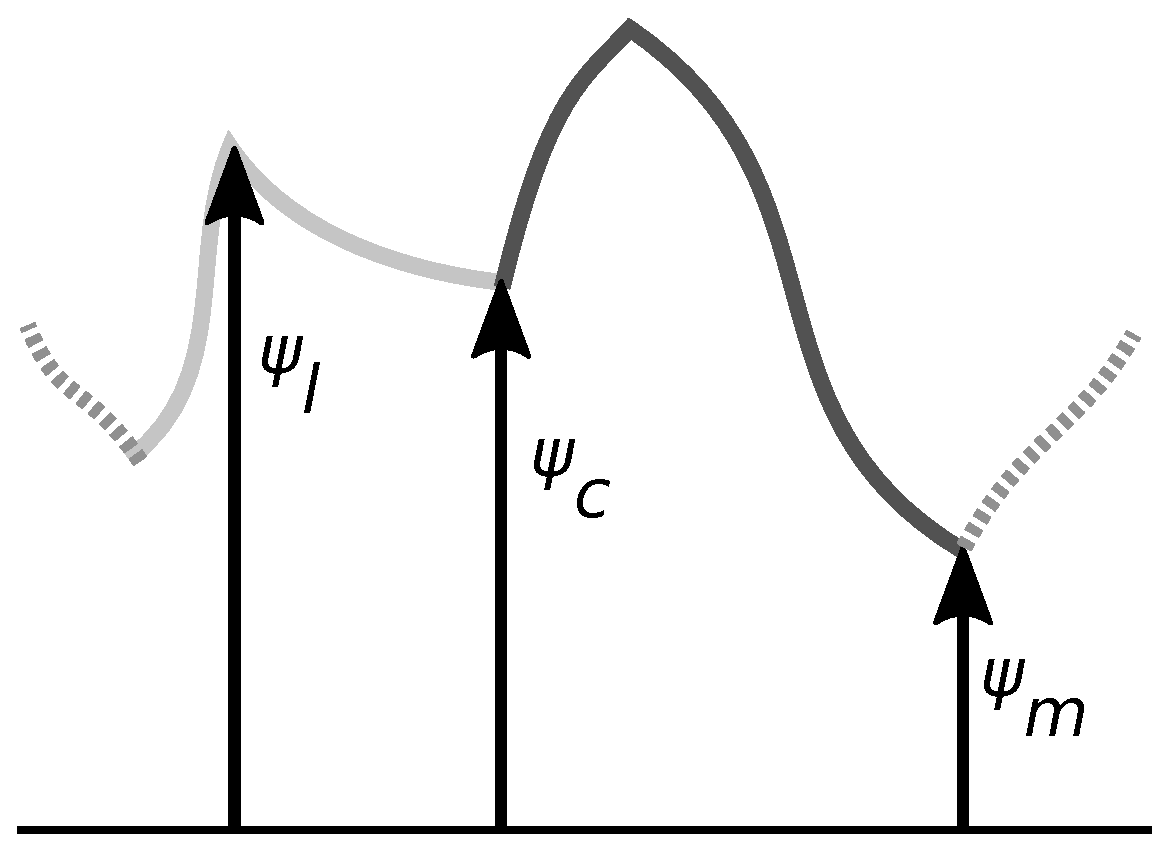
\includegraphics[width=0.40 \textwidth]{cols.eps}
 \caption{One-dimensional sketch of the different heights used in the merging algorithm, $\psi_c$, $\psi_l$ and $\psi_m$.}
 \label{fig:cols}
\end{figure}

The criterion used for merging is

\begin{equation}
\frac{\psi_l-\psi_c}{\psi_l-\psi_m}<=f
\end{equation}

Here $f$ is a parameter between 0 and 1: in our case it is set to 0.7. In the algorithm, $f$ is the only tunable parameter. In order to uniquely define the result, the order in which merges take place also matters. Here, we start with the highest col and process the cols in descending order.

As a sanity check, we considered the number of clouds in a field that contained a number of duplicates of the cloud field from a single simulation side by side. This resulted in a number of clouds that was the correct multiple of that of the original cloud field.

\end{document}
